\section{Related work}
This section discusses earlier created software and articles that are related to the goals of Tsukiji.

\subsubsection*{$\bullet$ pyLOB}
PyLOB \cite{pyLOB} is an open source project that simulates a financial exchange.
It does this by keeping an order-book that contains all previous made bids and asks and whenever two offers match, it automatically simulates a trade and removes the offers from the orderbook.
While PyLOB is not decentralised, the simulation helps understand how bids asks, and matching trades works.
It also offered a large set of offers from a real exchange, which can be used in different simulations.
\subsubsection*{$\bullet$ BarterCast}
BarterCast \cite{bartercast} is a fully distributed system that manages reputation of peers among a network. 
It uses the epidemic, also called gossip, protocol to spread information about the amount of data uploaded and downloaded by every peer.
Users uploading data use this information to decide who gets priority on receiving files.
Peers that have a better reputation of uploading get more slots to download from, since more peers are willing to share their data with them.
We used the same epidemic communication protocol in Tsukiji as scalable messaging solution. \\
\\
The following projects were found later in the development and their ideas could no longer be implemented in Tsukiji. 
They are nonetheless closely related projects and are worth mentioning.
\subsubsection*{$\bullet$ Bitmarkets}
Bitmarkets\cite{bitmarkets} is an open source project that includes a client and a protocol.
The client is a free OSX app for a decentralised marketplace that has users communicate using Bitmessage \cite{bitmessage} to hide the identity of the creator of a message.
These messages are sent to other users via the Tor\cite{tor} network.
This way both the identity as the location of the originator are hidden.
All that is visible is a public key generated by Bitmessage that can be used to reply on.
Payments are done using the multi-signature transactions of bitcoin.
This requires both parties to sign a transaction before the BitCoins are moved from wallet to wallet.
The issue with this mobile app is that apart from the solid transaction, there is no system in place that guarantees the seller actually sending the bought product.
\subsubsection*{$\bullet$ OpenMarket}
OpenMarket \cite{openmarket} claims to be another BitCoin-based decentralized market.
Rather than a large marketplace of buyers and sellers, OpenMarket lets people set up their own webshop by running one command.
This command creates a locally hosted website that support all functionality one would expect of a webshop.
Items to be sold can be added to the store with images and prices. 
Potential buyers can go to this site and browse the catalog of this particular seller.
Whenever the buyer wants to buy an item, it can add the item to a shopping cart and can checkout the whole cart.
Paying for the items happens is handled by the BitCoin network.
\begin{figure}[H]
  \centering
  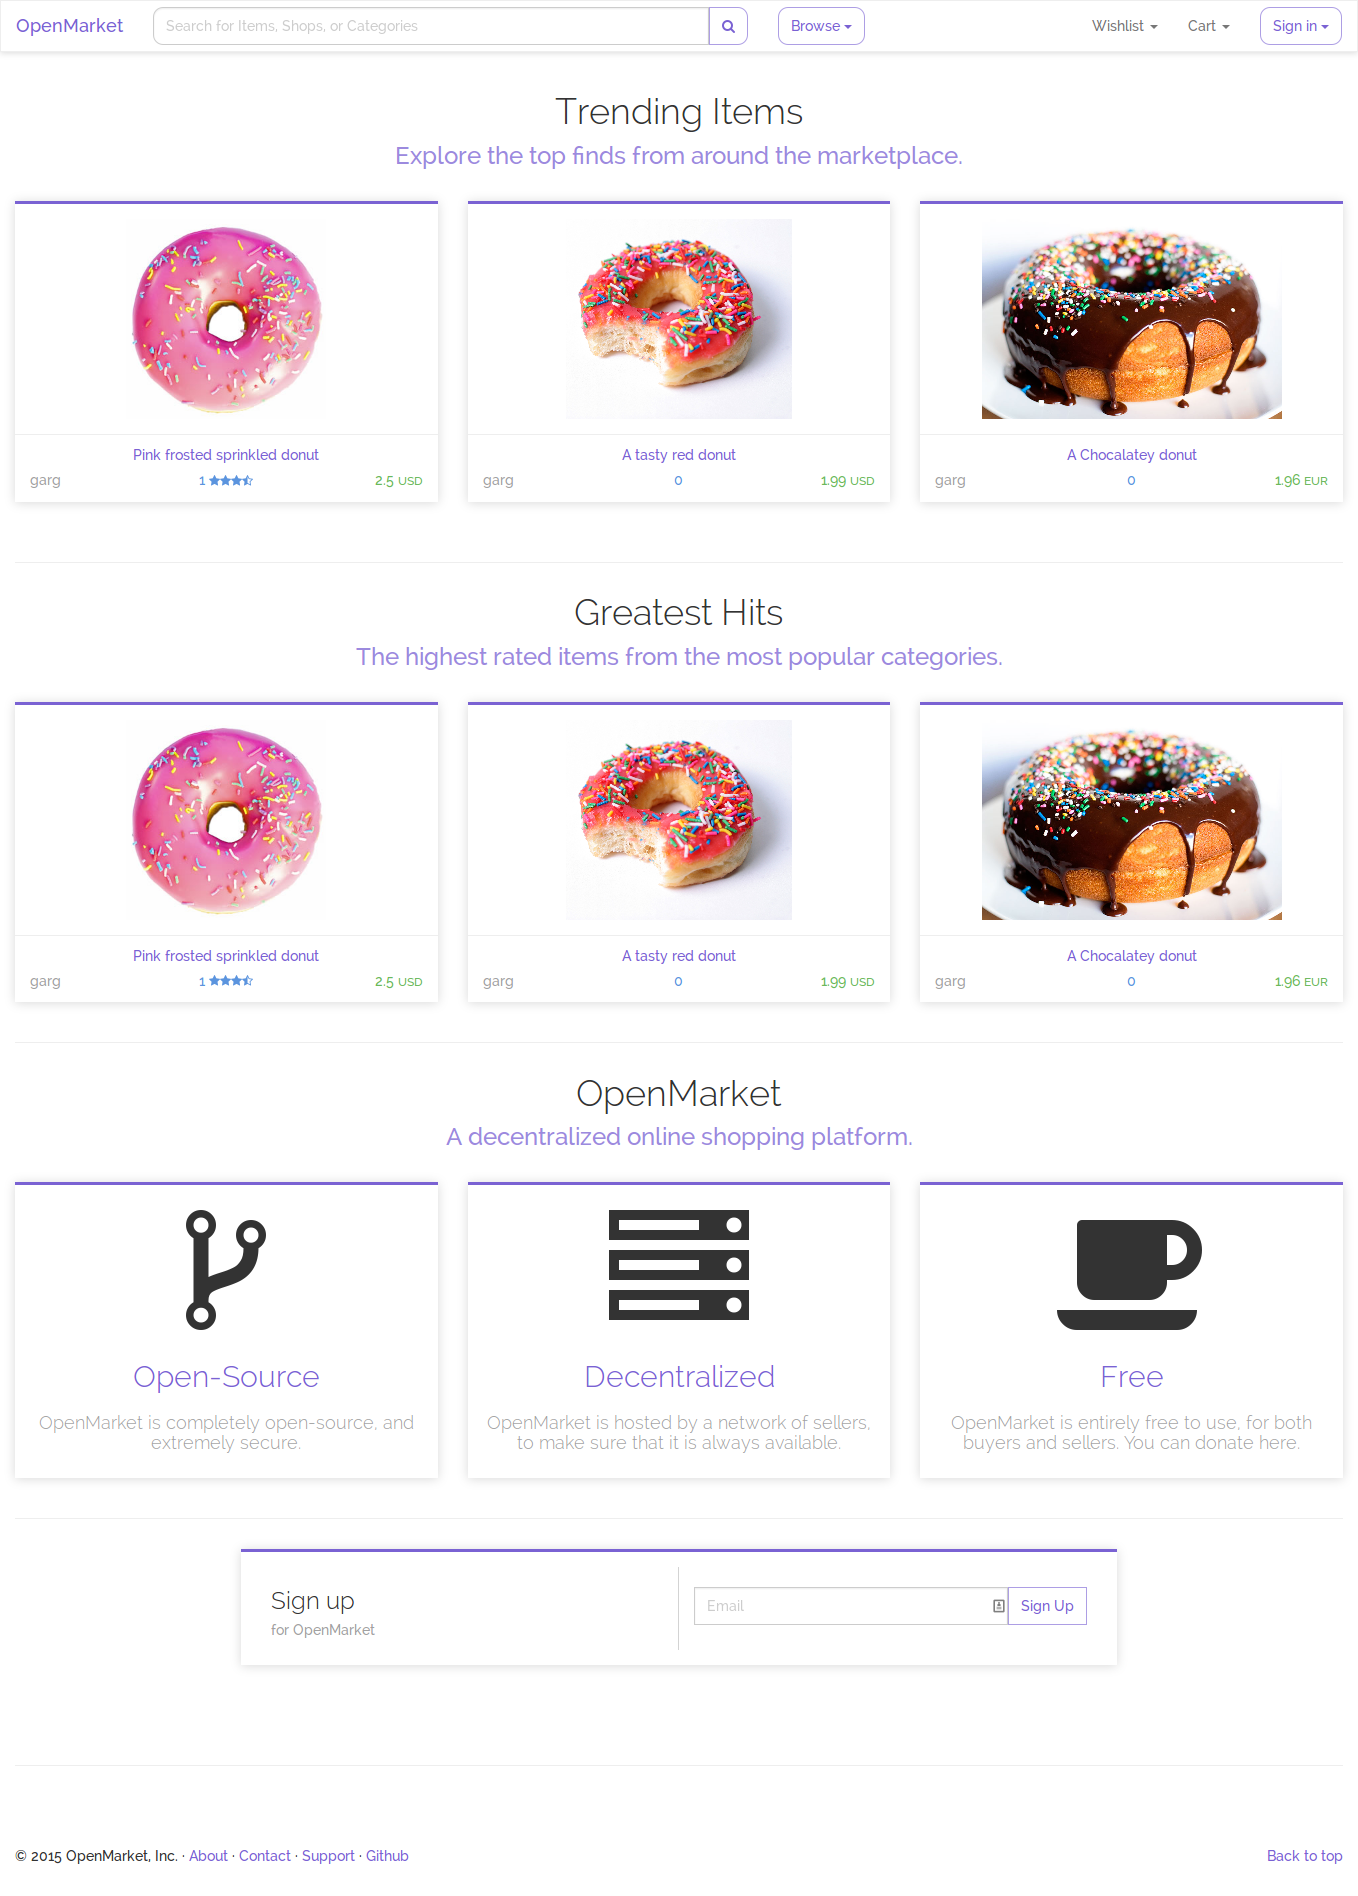
\includegraphics[scale=0.2]{openmarket}
  \caption{Example of a webstore created by OpenMarket}
  \label{openmarketfig}
\end{figure}
The problem with this implementation is that it is not truly one large marketplace without a central server, it is simple a lot of very small selling points running on very small servers.
There is no network, just a large amount of separate websites.
\subsubsection*{$\bullet$ OpenBazaar}
OpenBazaar \cite{bazaar} is also a decentralised marketplace where goods are traded with BitCoin.
It uses a Distributed Hast Table to connect peers in a scalable manner.
The software opens a webpage that represents the bazaar users can create their own shops on the bazaar.
Users can visit other shops and buy items from them, or simply wait until their something is bought from their own shop.
Items sold are hashed and this hash is used to create a contract.
Whenever someone buys the item, they sign the contract and send it to the seller.
The seller then in turn sends it to an independent third person on the network.
This escrow signs the contract and the buyer send bitcoin to a multisig deposit that can only be opened by at least two of the three keys.
Now, whenever a party lies about sending or receiving the item, they can attempt to prove this to the escrow and when the majority agree on the state of things, the bitcoins in the multisig deposit are sent to either the seller if everything is gone well, or returned to the buyer, if the product was not shipped.
While this is a great structure to reduce trust issues between parties, it is reliant on BitCoin. Non-digital currency cannot be easily locked away and retrieved.